% LuaLaTeX

\documentclass[a4paper, twoside, 12pt]{article}
\usepackage[latin]{babel}
%\usepackage[landscape, left=3cm, right=1.5cm, top=2cm, bottom=1cm]{geometry} % okraje stranky
\usepackage[portrait, a4paper, mag=1300, truedimen, left=0.8cm, right=0.8cm, top=0.8cm, bottom=0.8cm]{geometry} % okraje stranky

\usepackage{fontspec}
\setmainfont[FeatureFile={junicode.fea}, Ligatures={Common, TeX}, RawFeature=+fixi]{Junicode}
%\setmainfont{Junicode}

% shortcut for Junicode without ligatures (for the Czech texts)
\newfontfamily\nlfont[FeatureFile={junicode.fea}, Ligatures={Common, TeX}, RawFeature=+fixi]{Junicode}

\usepackage{multicol}
\usepackage{color}
\usepackage{lettrine}
\usepackage{fancyhdr}

% usual packages loading:
\usepackage{luatextra}
\usepackage{graphicx} % support the \includegraphics command and options
\usepackage{gregoriotex} % for gregorio score inclusion
\usepackage{gregoriosyms}
\usepackage{wrapfig} % figures wrapped by the text
\usepackage{parcolumns}
\usepackage[contents={},opacity=1,scale=1,color=black]{background}
\usepackage{tikzpagenodes}
\usepackage{calc}
\usepackage{longtable}

\setlength{\headheight}{12pt}

% Commands used to produce a typical "Conventus" booklet

\newenvironment{titulusOfficii}{\begin{center}}{\end{center}}
\newcommand{\dies}[1]{#1

}
\newcommand{\nomenFesti}[1]{\textbf{\Large #1}

}
\newcommand{\celebratio}[1]{#1

}

\newcommand{\hora}[1]{%
\vspace{0.5cm}{\large \textbf{#1}}

\fancyhead[LE]{\thepage\ / #1}
\fancyhead[RO]{#1 / \thepage}
\addcontentsline{toc}{subsection}{#1}
}

% larger unit than a hora
\newcommand{\divisio}[1]{%
\begin{center}
{\Large \textsc{#1}}
\end{center}
\fancyhead[CO,CE]{#1}
\addcontentsline{toc}{section}{#1}
}

% a part of a hora, larger than pars
\newcommand{\subhora}[1]{
\begin{center}
{\large \textit{#1}}
\end{center}
%\fancyhead[CO,CE]{#1}
\addcontentsline{toc}{subsubsection}{#1}
}

% rubricated inline text
\newcommand{\rubricatum}[1]{\textit{#1}}

% standalone rubric
\newcommand{\rubrica}[1]{\vspace{3mm}\rubricatum{#1}}

\newcommand{\notitia}[1]{\textcolor{red}{#1}}

\newcommand{\scriptura}[1]{\hfill \small\textit{#1}}

\newcommand{\translatioCantus}[1]{\vspace{1mm}%
{\noindent\footnotesize \nlfont{#1}}}

% pruznejsi varianta nasledujiciho - umoznuje nastavit sirku sloupce
% s prekladem
\newcommand{\psalmusEtTranslatioB}[3]{
  \vspace{0.5cm}
  \begin{parcolumns}[colwidths={2=#3}, nofirstindent=true]{2}
    \colchunk{
      \input{#1}
    }

    \colchunk{
      \vspace{-0.5cm}
      {\footnotesize \nlfont
        \input{#2}
      }
    }
  \end{parcolumns}
}

\newcommand{\psalmusEtTranslatio}[2]{
  \psalmusEtTranslatioB{#1}{#2}{8.5cm}
}


\newcommand{\canticumMagnificatEtTranslatio}[1]{
  \psalmusEtTranslatioB{#1}{temporalia/extra-adventum-vespers/magnificat-boh.tex}{12cm}
}
\newcommand{\canticumBenedictusEtTranslatio}[1]{
  \psalmusEtTranslatioB{#1}{temporalia/extra-adventum-laudes/benedictus-boh.tex}{10.5cm}
}

% volne misto nad antifonami, kam si zpevaci dokresli neumy
\newcommand{\hicSuntNeumae}{\vspace{0.5cm}}

% prepinani mista mezi notovymi osnovami: pro neumovane a neneumovane zpevy
\newcommand{\cantusCumNeumis}{
  \setgrefactor{17}
  \global\advance\grespaceabovelines by 5mm%
}
\newcommand{\cantusSineNeumas}{
  \setgrefactor{17}
  \global\advance\grespaceabovelines by -5mm%
}

% znaky k umisteni nad inicialu zpevu
\newcommand{\superInitialam}[1]{\gresetfirstlineaboveinitial{\small {\textbf{#1}}}{\small {\textbf{#1}}}}

% pars officii, i.e. "oratio", ...
\newcommand{\pars}[1]{\textbf{#1}}

\newenvironment{psalmus}{
  \setlength{\parindent}{0pt}
  \setlength{\parskip}{5pt}
}{
  \setlength{\parindent}{10pt}
  \setlength{\parskip}{10pt}
}

%%%% Prejmenovat na latinske:
\newcommand{\nadpisZalmu}[1]{
  \hspace{2cm}\textbf{#1}\vspace{2mm}%
  \nopagebreak%

}

% mode, score, translation
\newcommand{\antiphona}[3]{%
\hicSuntNeumae
\superInitialam{#1}
\includescore{#2}

#3
}
 % Often used macros

\setlength{\columnsep}{15pt} % prostor mezi sloupci

%%%%%%%%%%%%%%%%%%%%%%%%%%%%%%%%%%%%%%%%%%%%%%%%%%%%%%%%%%%%%%%%%%%%%%%%%%%%%%%%%%%%%%%%%%%%%%%%%%%%%%%%%%%%%
\begin{document}

% Here we set the space around the initial.
% Please report to http://home.gna.org/gregorio/gregoriotex/details for more details and options
\grechangedim{afterinitialshift}{2.2mm}{scalable}
\grechangedim{beforeinitialshift}{2.2mm}{scalable}
\grechangedim{interwordspacetext}{0.20 cm plus 0.15 cm minus 0.05 cm}{scalable}%
\grechangedim{annotationraise}{-0.2cm}{scalable}

% Here we set the initial font. Change 38 if you want a bigger initial.
% Emit the initials in red.
\grechangestyle{initial}{\color{red}\fontsize{34}{34}\selectfont}

\renewcommand{\headrulewidth}{0pt} % no horiz. rule at the header
\pagestyle{empty}

\cantusCumNeumis

\grechangedim{spaceabovelines}{0.2cm}{scalable}%

\begin{center}


\includegraphics[width=5cm]{svhavel.jpg}

\vspace{5mm}

{\fontsize{32pt}{38.4pt} \textsc{Instalace zvonu svatý Václav}}

{\large ulitého z iniciativy Charty 77\\
na poděkování Bohu za dar svobody\\
a ke cti těch, kdo se o ni zasloužili,\\
včetně pana prezidenta Václava Havla\\
}

\vfill

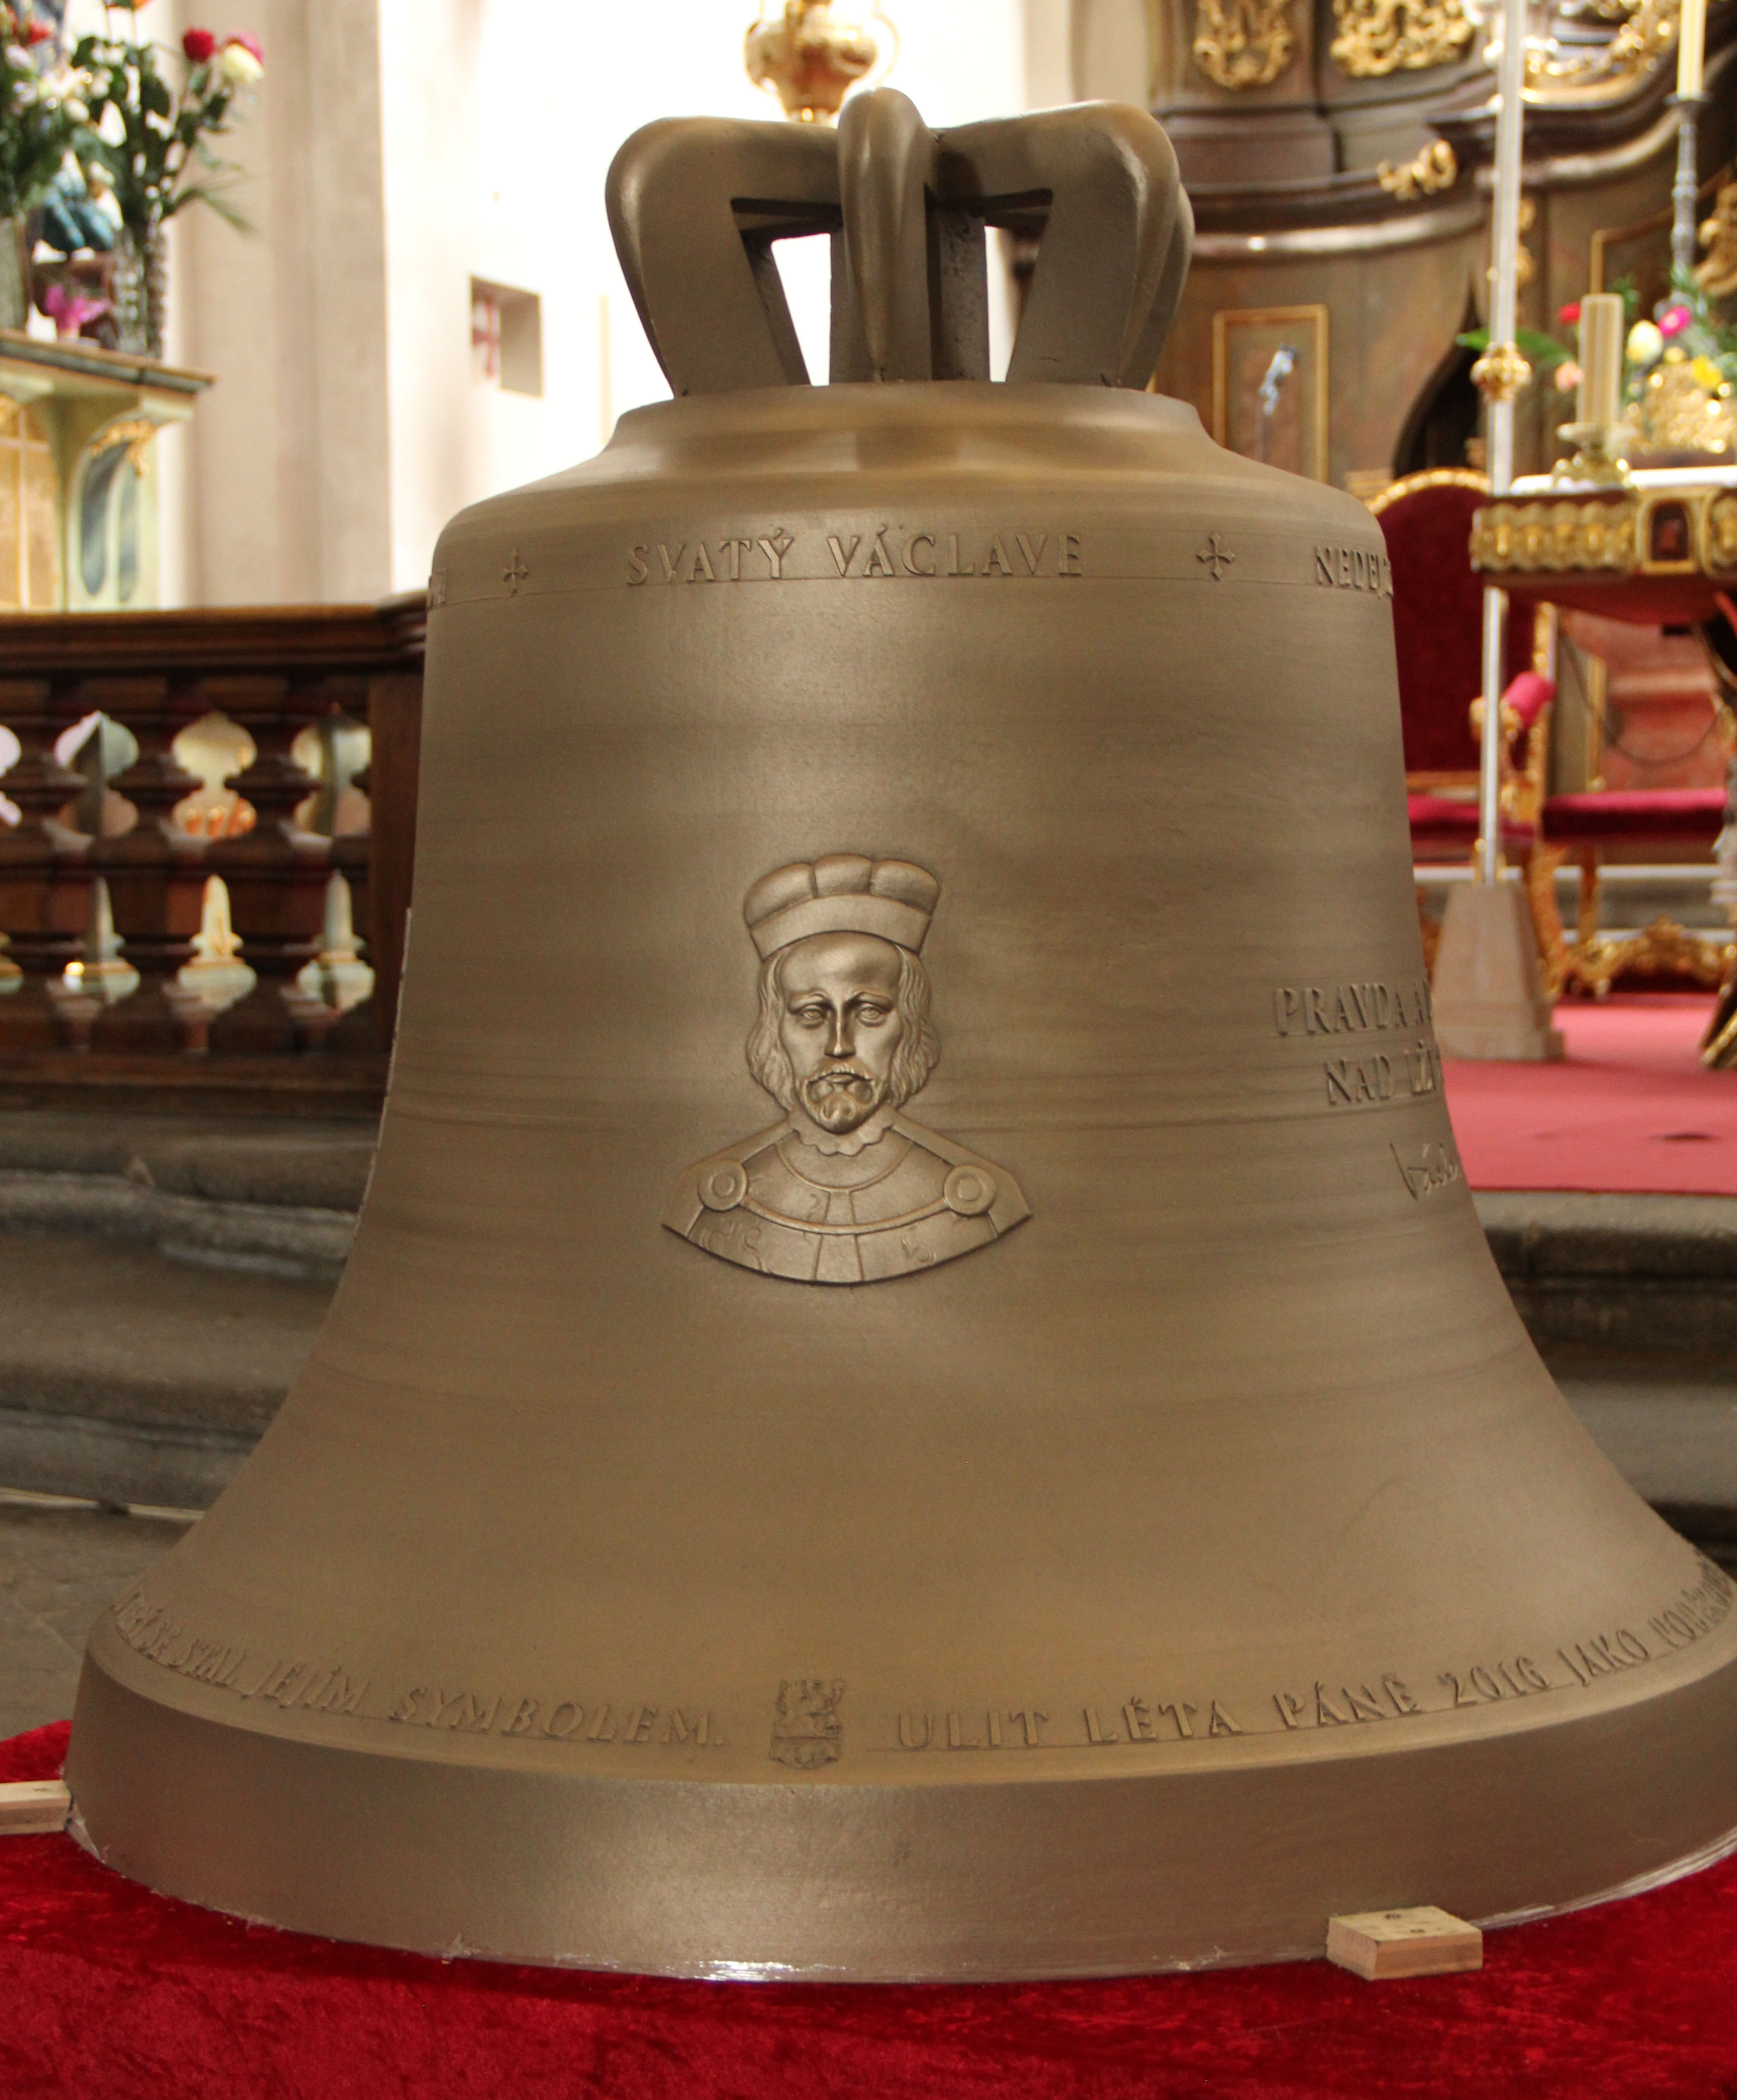
\includegraphics[width=7cm]{campana.jpg}

\vfill

{\large \textsc{Všem dárcům upřímně děkujeme…}}

{\large kostel sv. Havla v Praze 5.3.2017}

\end{center}

\vspace{5mm}

%\vfill
\pagebreak

\noindent \includegraphics[scale=0.77, clip, trim= 8mm 140mm 0mm 7mm]{temporalia/dekovnapiseni}

\vfill

\noindent \includegraphics[scale=0.77, clip, trim= 8mm 260mm 0mm 7mm]{temporalia/trishagion}

\vfill

\vspace{-5mm}

\begin{center}
{\fontsize{13pt}{14pt} \textbf{Tractus Qui Habitat}}
\end{center}

\vspace{-10mm}

\scriptura{Ps. 90, 1-7.11-16; \textbf{L40}}

\vspace{-5mm}

\gresetnabcfont{grelaon}{8}
\grechangestaffsize{11}

\antiphona{TR. II}{temporalia/tractus-QuiHabitat.gtex}

\vspace{-2mm}

\begin{translatioMulticol}{2}
Kdo žije pod ochranou Nejvyššího,~\grestar{}\\
přebývá v stínu Všemohoucího,\\
ať říká Pánu: ,,Tys mé útočiště,~\grestar{}\\
můj hrad a Bůh můj, v nějž mám důvěru.`` –\\
Vždyť on tě zachraňuje z tenat lovců,~\grestar{}\\
před slovem, které zkázu přináší.\\
On zastíní tě svými perutěmi,~\grestar{}\\
pod jeho křídly dojdeš ochrany.\\
Nebudeš strachovat se nočních příšer~\grestar{}\\
a šípů, které za dne létají,\\
nákazy, která v temnotách se plíží,~\grestar{}\\
moru, jenž řádí za bílého dne. –\\
I když jich padne po tvém boku tisíc,~\grestar{}\\
ba deset tisíc po tvé pravici,\columnbreak

záhuba přesto tebe nedosáhne.\\
Vždyť kvůli tobě andělům dal příkaz,~\grestar{}\\
na všech tvých cestách být ti ochránci. –\\
A proto budou na rukou tě nosit,~\grestar{}\\
aby ses neporanil o kámen.\\
A budeš kráčet po hadech a štírech~\grestar{}\\
a lva i draka klidně zašlápneš. –\\
,,Že je mi oddán, já ho vysvobodím,~\grestar{}\\
ochráním, že se k mému jménu zná.\\
A vyslyším ho, když mě bude vzývat,~\gredagger{}\\
budu s ním v každém jeho soužení,~\grestar{}\\
zachráním ho a ke cti pozvednu.\\
Dosyta obdařím ho dlouhým věkem~\grestar{}\\
a svoji spásu mu dám uvidět.``
\end{translatioMulticol}


\vfill
%\pagebreak

\noindent \includegraphics[scale=0.77, clip, trim= 10mm 67mm 0mm 7mm]{temporalia/svatyvaclave}

\vfill
\pagebreak

\noindent \includegraphics[scale=0.77, clip, trim= 10mm 0mm 0mm 232mm]{temporalia/svatyvaclave}

\vfill
%\pagebreak

\noindent \includegraphics[scale=0.77, clip, trim= 8mm 235mm 0mm 7mm]{temporalia/tedeum}

\vspace{-5mm}

\begin{translatioMulticol}{3}
Vše, co jen chválit může,\\
cherubové, serafové,\\
chválí tě velký Bože,\\
nebe, země, zástupové,\\
ode všech jsi nazýván:\\
Svatý, Svatý, Svatý Pán.\\
\\
Svatý Pán Bůh Sabaoth,\\
Svatý, jenž řídí národy,\\
jenž pomáhá z běd a psot.\\
Nebe, zem, povětří, vody\\
plné jsou cti, chvály tvé,\\
neb vše tvoje dílo je.\\
\\
Apoštolů slavný sněm\\
a proroků řad veliký\\
posílá v plesání svém\\
k trůnu tvému vroucí díky;\\
kolik je mučedníků,\\
tolik chvalořečníků.\\
\\
Po všem okrsku země\\
tobě, Otče, velcí, malí,\\
kdož jsou tvé svaté plémě,\\
vděčně prozpěvují chvály,\\
vzdávají čest i Synu\\
na trůnu sedícímu.\columnbreak

Též i Duchu Svatému,\\
který svatá naučení\\
uděluje každému\\
a v smutku je utěšení,\\
lid křesťanský se klaní,\\
všude jeho chvála zní.\\
\\
Ty, Otče věčný Synu,\\
vtělil ses, sestoupiv z nebe,\\
chtě smazat naši vinu\\
vydals na smrt kříže sebe;\\
milost jsi nám vydobyl,\\
od hříchu osvobodil.\\
\\
Tebou je všem, kdo věří,\\
nebes brána otevřena,\\
s důvěrou kdo k tobě zří,\\
zastáncem tě u Otce má.\\
Že přijdeš svět souditi,\\
máme mít vždy v paměti.\\
\\
Buď milostiv dětem svým,\\
požehnej dědictví svému,\\
veď nás světlem nebeským\\
a povyš až k trůnu svému,\\
ať tě, plni vděčnosti,\\
chválíme na věčnosti.\columnbreak

Přispěj zatím k pomoci\\
drahou krví vykoupeným,\\
chraň a braň je svou mocí,\\
přičti ke svým vyvoleným;\\
po časném pak bloudění\\
přiveď nás ke spasení.\\
\\
To buď naše snažení:\\
tebe a tvé jméno vzývat,\\
čest a díkůčinění\\
po všechny dny tobě zpívat.\\
Rač od hříchů chránit nás\\
jak dnes, tak po všechen čas.\\
\\
Pane, smiluj, smiluj se,\\
buď s námi tvé požehnání;\\
oč prosíme, staniž se\\
podle našeho doufání.\\
Kdo v tě doufá samého,\\
neopustíš žádného.
\end{translatioMulticol}


\end{document}
